A la hora de lanzar todos los rayos de la simulación y su evaluación se presentan dos vías: la ejecución en serie en una CPU usual y la ejecución en paralelo en una GPU.

Aunque ambas opciones compartan gran parte de los cálculos, las diferentes estructuras entre los dispositivos hacen que se presenten diferencias a la hora de implementar la simulación.

\subsection{Elementos comunes}

Partiendo de las bases descritas en la sección anterior la simulación consistirá, de forma general, en lanzar rayos y acumular los resultados de los receptores.

Aprovechando las ventajas de la programación orientada a objetos, se considerarán los siguientes clases:
\begin{itemize}
    \item \textbf{Rayo} Esta clase contendrá el punto de partida y el vector de dirección del rayo, así como la potencia en el origen.
    \item \textbf{Pared} En esta clase se incluirán los cuatro puntos de los extremos de la pared, a partir de los que se calculará su normal, también almacenada. Además, contendrá el valor de permeabilidad dieléctrica de su material. Implementará métodos para determinar si un rayo la impacta, y obtener tanto el punto de impacto como el rayo reflejado.
    \item \textbf{Receptor} Esta clase incluye el origen de la esfera y su radio. Al igual que la clase de las paredes implementará métodos para determinar si un rayo la impacta, y obtener la potencia teniendo en cuenta el patrón de emisión de la antena que modeliza.
\end{itemize}

La simulación comienza con la obtención del entorno virtual.
A partir de medidas en el entorno real, se escriben en un archivo las esquinas de todas las paredes de entorno, así como los límites de los objetos.

Con estas esquinas se construye un vector con los objetos de paredes, creados a partir de estas esquinas.
Este vector constiuirá el mapa de la simulación.

Una vez se ha creado el mapa se crean los receptores, con la posición y su distancia.
Aunque la implementación permite cualquier radio, en este caso se limitó a $2.5$cm.

El siguiente paso será leer el patrón de radiación de las antenas.
Ya que para esta simulación el de el emisor y el receptor es el mismo, solo se hará en una ocasión, y se utilizarán también estos datos para la generación de rayos.

Este patrón, como se explicaba en la Sección~\ref{sec:antenas}, está generado directamente por MATLAB, y su formato es el de una matriz en el que cada uno de los ejes indica un ángulo.
Su lectura y uso sigue el mismo formato.

Una vez cargados todos los datos, se inicia el bucle principal, deberá recorrer el ángulo azimutal y el ángulo de elevación avanzando con un cierto valor prefijado en ambos.
En las subsecciones posteriores se profundizará en la evaluación de cada rayo.

Una vez se han lanzado todos los rayos se acumulan los resultados --de nuevo, en las siguientes subsecciones se discutirá en detalle la estructura de memoria para estos resultados-- y se escriben en un archivo para su análisis posterior.

El Algoritmo~\ref{alg:euclid} recoge en pseudocódigo todo el proceso.

% \ref{sec:paredes}

% Las clases de las paredes y los receptores implementarán métodos que tengan de entrada un cierto rayo y que determinarán si habrá algún impacto entre ellos.

% A la hora de almacenar los datos de los receptores no es posible acumular los valores de todos los rayos impactados ya que daría valores muy altos totalmente irreales.
% El hecho de que muchos de los rayos impacten contra los receptores es fruto de la modelización como esfera, dando más volumen del que realmente tiene la esfera.

% Por ello, se dividirá el reconocimiento de impactos dependiendo de los rebotes que haya recibido.
% De esta forma se podrán separar los rayos que se reciben de forma directa de los rebotados.

% A la hora de registrar la potencia recibida, para cada uno de los rebotes que ha sufrido el rayo, se elegirá aquel con una potencia mayor, al ser el que impacta de forma más directa con la esfera receptora, comportamiento buscado.

% Estos valores se registrarán en una matriz en la que se considera a cada fila como cada receptor, y cada columna como estos valores de rebotes.
% Así, tras finalizar la evaluación de rayos se acumularán todos los valores en cada fila, siendo el resultado final para cada receptor.

\begin{algorithm}
    \caption{Bucle Principal}
    \label{alg:euclid}
    \begin{algorithmic}[1]
        \State Leer parámetros.
        \State Cargar mapa.
        \State Colocar receptores.
        \For{azimut $\in [0, 360)$}\Comment{Se evaluan los ángulos sumando un cierto paso fijado en los parámetros.}
            \For{elev $\in [90, -90]$}
                \State eval\_ray(azimut, elev, pot, data)
            \EndFor
        \EndFor

        \Comment{Data indica la matriz donde se acumulan los resultados.}
        \For{$i\gets 0, rows(data)$}
            \ForAll{$j\gets 1, cols(data)$}
                \State data[i][0] $\gets$ data[i][0] + data[i][j]
            \EndFor
        \EndFor

        \State write\_results(file, data)
    \end{algorithmic}
\end{algorithm}

\subsubsection*{Evolución de cada rayo}

El lanzamiento y evolución de cada rayo tiene varias fases a discutir.

En primer lugar, una vez se ha determinado la dirección de lanzamiento se debe calcular la potencia a emitir.
Habiendo importado la direccionalidad de la antena de emisión, se realiza una interpolación bidimiensional\footnote{En este caso esta interpolación ha sido bilineal. Aunque es posible obtener unos valores más precisos con métodos de mayor orden, partiendo de puntos separados solo un grado en ambos ángulos esta elección proporciona valores aceptables sin tener que abordar las condiciones de contorno en los extremos.} para estimar el valor correspodiente.

Una vez se ha lanzado, cada rayo buscará en primer lugar la pared contra la que impactará.
Esta pared será la que proporcione una distancia de impacto menor.

Tras ello, se buscarán los receptores contra los que impactará el rayo.
En este caso se recorrerán todos los receptores colocados, y solo se considerarán como impactados aquellos para los que la distancia de impacto sea menor que la distancia de impacto contra la pared.

Esta consideración se produce para evitar el impacto contra receptores que se encuentren detrás de una pared u objeto.

Una vez se han recorrido ambos elementos, se habrá completado la interacción del rayo con el medio.
Se determinará su punto de impacto: si lo hay, será el punto donde se generarán el rayo transmitido y el rayo reflejado.
Se evaluará solo el rayo transmitido, por lo que el reflejado tendrá que ser almacenado.

Este almacenamiento se hará en forma de pila, de tal forma que los rayos añadidos más recientemente serán los primeros en ser evaluados.
Esta elección es totalmente arbitraria: todos los rayos son independientes entre sí.

Para optimizar el uso de memoria de la pila se reservará toda la memoria que se podría usar antes de iniciar el bucle y así no necesitar movimientos posteriores.
El tamaño necesario vendrá determinado por el número de rebotes que se quieran registrar.

\begin{figure}[H]
    \centering
    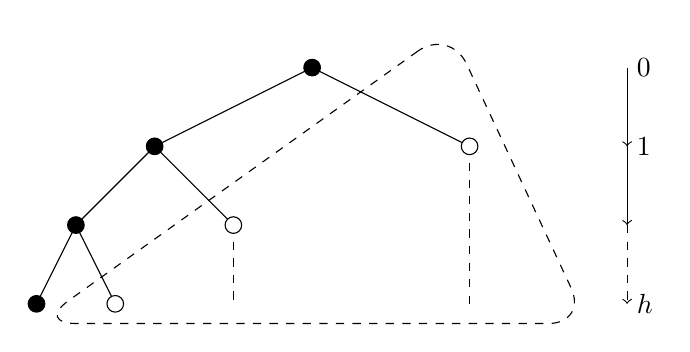
\begin{tikzpicture}

    % Conexiones
    \draw (0,0) -- (-2,-1);
    \draw (0,0) -- (2,-1);

    \draw (-2,-1) -- (-3,-2);
    \draw (-2,-1) -- (-1,-2);

    \draw (-3,-2) -- (-3.5,-3);
    \draw (-3,-2) -- (-2.5,-3);

    \draw[dashed] (2,-1) -- (2,-3);
    \draw[dashed] (-1,-2) -- (-1,-3);


    % Puntos
    \filldraw (0,0) circle [radius=3pt, fill=black];

    \filldraw (-2,-1) circle [radius=3pt, fill=black];
    \filldraw[draw=black, fill=white] (2,-1) circle [radius=3pt];

    \filldraw (-3,-2) circle [radius=3pt, fill=black];
    \filldraw[draw=black, fill=white] (-1,-2) circle [radius=3pt];

    \filldraw (-3.5,-3) circle [radius=3pt, fill=black];
    \filldraw[draw=black, fill=white] (-2.5,-3) circle [radius=3pt];

    % Niveles
    \draw[->] (4,0) -- (4,-1);
    \node[anchor=west] at (4,0) {0};

    \draw[->] (4,-1) -- (4,-2);
    \node[anchor=west] at (4,-1) {1};


    \draw[dashed, ->] (4,-2) -- (4,-3);
    \node[anchor=west] at (4,-3) {$h$};

    % Envoltorio

    \draw[dashed] [rounded corners=0.5cm] (1.75,0.5) -- (-3.5,-3.25)[rounded corners=0.5cm] -- (3.5,-3.25) -- cycle;


\end{tikzpicture}
    \caption{Árbol generado por los impactos de los rayos hasta llegar a $h$ impactos. Los puntos negros indican los rayos reflejados, evaluados inmediatamente; los blancos, los transmitidos. En la línea punteada, el número máximo de rayos a almacenar.}
    \label{fig:memoria_pila}
\end{figure}

En la Figura~\ref{fig:memoria_pila} se indica el árbol generado por un rayo, donde en cada impacto nacen dos rayos.
Considerando que siempre se evalúa el rayo reflejado --en esta representación, el camino de la izquierda-- podría parecer que se deberá reservar memoria para todos los rayos restantes, pero es posible un uso menor.

Los rayos guardados en la pila no son evaluados de forma inmediata, así que los rayos que se generan no se conocerán hasta que se llegue a su nodo.
Es decir, el número de rayos en la pila no llegará nunca a ser tan alto, aunque es necesario dar un número de elementos a reservar.

Para ello se asumirá que es imprescindible guardar todos los rayos recogidos en la línea punteada.
Estos serán todos los elementos del árbol ($\sum_h 2^h$) menos el número de niveles que tenga, que será $h+1$ teniendo en cuenta que tal y como se indica, se ha empezado a contar desde el cero y así
\begin{equation}
    \text{\# Rayos a guardar} = \sum_{h=0}^{\infty} 2^h - (h+1)
\end{equation}

El Algoritmo~\ref{alg:ray} contiene, en pseudocódigo, la subroutina que evalúa cada rayo tal y como se ha descrito en la sección.

\begin{algorithm}
    \caption{Bucle que evalúa cada rayo}
    \label{alg:ray}
    \begin{algorithmic}[1]
        % \State Añadir pareja \{rayo inicial, 0\} a la pila.
        
        \While{Tamaño pila > 0}
            \State reb $\gets$ segundo valor de la pareja \{rayo, rebote\}.

            \ForAll{Paredes}
                \State hit\_dist $\gets$ INFINITY
                \State wall\_hit $\gets$ -1
                \If{Pared golpeada}
                    \If{dist < hit\_dist}
                        \State hit\_dist $\gets$ dist
                        \State wall\_hit $\gets$ pared
                    \EndIf
                \EndIf
            \EndFor

            \ForAll{Receptores}
                \State hit\_dist $\gets$ INFINITY
                \State power $\gets$ 0
                \If{Receptor golpeado}
                    \If{hit\_power > power AND dist < hit\_dist}
                        \State hit\_power $\gets$ power
                    \EndIf
                \EndIf
            \EndFor

            \If{power > CUTOFF\_POWER AND reb < MAX\_REBOUND}
                \State \{rayo, rebote\} $\gets$ \{ rayo\_reflejado, reb+1\}
                \State Añadir \{ rayo\_transmitido, reb+1\} a la pila.
            \Else
                \State \{rayo, rebote\} $\gets$ último valor de la pila.
            \EndIf
        \EndWhile
    \end{algorithmic}
\end{algorithm}

\subsubsection*{Registro en los receptores}

Una vez los rayos se propagan de forma libre por el entorno se esparará a su impacto con cada uno de los receptores para registrar su efecto.

Hay que tener en cuenta que se busca sumar la potencia recibida en cada receptor por parte de todos los rayos que los cruzen, pero con un detalle: no se pueden registrar todos los rayos sin más.

Si se suma la potencia de cualquiera de los rayos que impactan contra un receptor se obtendrán potencias totales totalmente irreales, ya que, especialmente en el caso de receptores colocados a distancias cercanas al emisor, habrá una gran cantidad de rayos que, indicando un mismo frente de ondas, lleguen al impacto contra ellos.

Este comportamiento es completamente irreal, fruto de la aproximación de la antena como esferas.
El frente de ondas, representado por un solo rayo, solo debería cruzarla una vez y no un número mayor como ocurriría en este caso.

La misma situación se presenta en los rebotes, con lo que se podría acabar con un exceso de potencia tanto en los rayos que llegan de forma directa como en los que llegan tras la interacción con las paredes u objetos.

Para evitar esto solo se registrará el rayo con mayor potencia.
Debido al gran decaimiento de la potencia con la distancia, esto indicará el rayo que impacte de forma más directa contra la esfera.
En otro caso, la distancia adicional hará que su potencia sea menor.

Además, se tendrá la consideración de los rebotes sufridos por el rayo.
Si solo se toma el criterio anterior, solo se registrarían los rayos que impactan de forma directa.

Para solventar este problema se asociará cada rayo al número de rebotes que ha sufrido.
Así, una vez impacten con los receptores se considerará este valor, y cada vez que reboten contra algún objeto se actualizará.

Los resultados se almacenarán considerando una matriz con tantas filas como receptores y tantas columnas como número máximo de rebotes a registrar.
Cuando el cálculo finalice, se acumularán los resultados sumando los valores por filas en la primera columna obteniendo el resultado final de cada receptor.

\subsection{Implementación en serie}

La implementación en serie de la simulación para ser ejecutada en una CPU sigue el procedimiento explicado en esta sección.

Existirá una zona de memoria reservada para registrar los datos y simplemente se recurre a un doble bucle \textit{for} que irá completando los resultados evaluando cada par de ángulos avanzando con un cierto paso predefinido.

Ya que la evaluación de cada rayto se realizará de forma totalmente secuencial, no será necesario añadir ninguna consideración adicional.

\subsection{Implementación en paralelo}

El hecho de que los rayos lanzados sean independientes entre sí convierte en el bucle principal en el escenario perfecto para ser ejecutado de forma paralela, ya que cada iteración del bucle no se verá interrumpida por las demás.

Para esta paralelización se ha hecho uso de tarjetas gráficas, que cuentan con un gran número de núcleos de cómputo pero para las que hay que tener en cuenta su estructura de memoria.

En general, a la hora de paralelizar un algoritmo es necesario hacer duplicaciones de datos para evitar condiciones de carrera que proporcionen resultados erróneos.
En los casos de muy alta paralelización como este es posible encontrarse con ciertas limitaciones.

La tarjeta gráfica usada en este caso ha sido una Nvidia GTX1070, sobre la que es posible el uso de la librería de Nvidia CUDA.
Esta tarjeta cuenta con 1920 núcleos agrupados en 15 multiprocesadores.

La estrategia de paralelización consistirá en asignar un rayo a cada hilo, que contará con su matriz de datos correspondiente donde registrará los impactos para luego ser acumulada en los datos finales.

Las tarjetas gráficas agrupan sus hilos en bloques.
Los hilos que se encuentren en un mismo bloque pueden acceder a una cierta cantidad de memoria compartida de un acceso más rápido que la memoria global común.

Para reducir la necesidad de memoria y aprovechar esta característica la acumulación de los datos se producirá en dos fases: el cálculo de cada rayo --asignado a cada hilo-- volcará sus datos en la memoria compartida del bloque.
Una vez acaban todo los hilos del bloque, se acumulan los datos en la memoria global, donde se ha reservado espacio para cada bloque.

Debido a la herencia del uso de este tipo de dispositivos para trabajos de vídeo, es posible acceder a los hilos y bloques con dos índices, de forma similar a una matriz.
Esta característica será útil en este caso, en el que los rayos se lanzarán en torno a los dos ángulos de las coordenadas esféricas.

Así, se asociará la dirección $x$ al ángulo azimutal y la dirección $y$ a la elevación.

Queda determinar el número de hilos en cada bloque.
En general, la memoria disponible para su uso compartido es una cantidad baja.
En el caso de la tarjeta gráfica usada, es de 48 KB\cite{Nvidia}.

\begin{figure}[H]
    \centering
    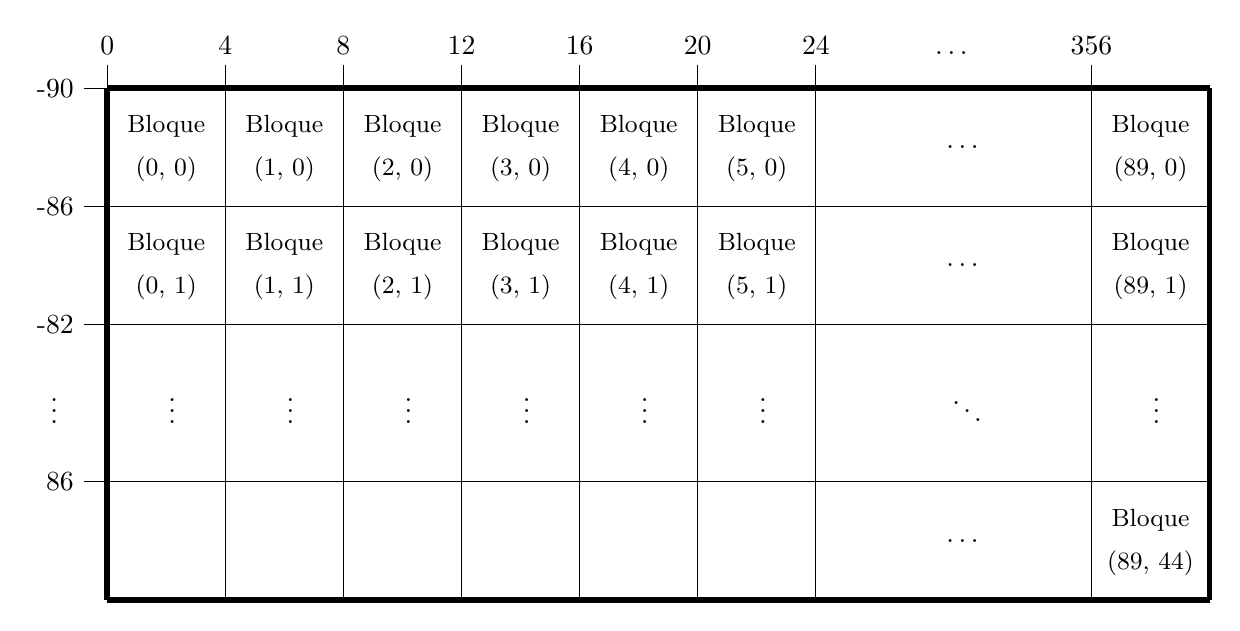
\begin{tikzpicture}
    \draw[line width=2pt] (0,0) -- (14,0);
    \draw[line width=2pt] (0,-6.5) -- (14,-6.5);
    \draw[line width=2pt] (0,0) -- (0,-6.5);
    \draw[line width=2pt] (14,0) -- (14,-6.5);

    % Labels
    \foreach \i in {0, 1.5, 3,...,10}
    {
        \draw (\i,0.3) -- (\i,-6.5);
        \pgfmathtruncatemacro{\label}{4*\i/1.5};
        \node[anchor=south] at (\i, 0.3) {\label \si{\degree}};
    }
    \draw (12.5,0.3) -- (12.5,-6.5);
    \node[anchor=south] at (12.5, 0.3) {356\si{\degree}};
    \node[anchor=south] at (10.75, 0.3) {\ldots};

    \foreach \i in {0, -1.5, -3}
    {
        \draw (-0.3, \i) -- (14, \i);
        \pgfmathtruncatemacro{\label}{90+4*\i/1.5};
        \node[anchor=east] at (-0.3, \i) {-\label \si{\degree}};
    }

    \draw (-0.3, -5) -- (14, -5);
    \node[anchor=east] at (-0.5, -4) {\vdots};
    \node[anchor=east] at (-0.3, -5) {86\si{\degree}};

    %Blocks
    \foreach \i in {1.5, 3, ...,10}
    {
        \pgfmathtruncatemacro{\bloquei}{\i/1.5 - 1};
        \foreach \j in {-1.5, -3}{
            \pgfmathtruncatemacro{\bloquej}{-\j/1.5-1};
            \node[anchor=south] at (\i-0.75, \j+0.75) {\small{Bloque}};
            \node[anchor=north] at (\i-0.75, \j+0.75) {\small{(\bloquei, \bloquej)}};

        }
        % \draw (\i,0.3) -- (\i,-6.5);
        % \pgfmathtruncatemacro{\label}{4*\i/1.5};
        
    }

    % Bloques extremo izquerda
    \node[anchor=south] at (13.25, -0.75) {\small{Bloque}};
    \node[anchor=north] at (13.25, -0.75) {\small{(89, 0)}};

    \node[anchor=south] at (13.25, -2.25) {\small{Bloque}};
    \node[anchor=north] at (13.25, -2.25) {\small{(89, 1)}};

    \node[anchor=south] at (13.25, -5.75) {\small{Bloque}};
    \node[anchor=north] at (13.25, -5.75) {\small{(89, 44)}};


    %Puntitos
    \foreach \i in {1.5, 3, ..., 10, 14}
    {
        \node[anchor=east] at (\i-0.5, -4) {\vdots};
    }

    \foreach \j in {0, -1.5, -5}
    {
        \node[anchor=east] at (11.25, \j-0.75) {\ldots};
    }

    \node[anchor=east] at (11.25, -4) {$\ddots$};


\end{tikzpicture}
    \vspace*{-0.75cm}
    \caption{Esquema con la asignación de ángulos a cada bloque de hilos.}
    \label{fig:CUDA_angulos}
\end{figure}

Esta cantidad no permite lanzar bloques con un número grande de hilos, aunque dependerá del número de receptores y los rebotes que se quieran registrar.
A modo de ejemplo, al colocar unos 40 receptores y registrar los rayos hasta 5 rebotes, con valores de precisión simple --es decir, 4 bytes--, podremos lanzar bloques con 60 hilos como máximo.

Para evitar futuras incompatibilidades en caso de elegir valores mayores en alguno de estos dos parámetros, se han elegido el mínimo valor de hilos posible.
La elección es la siguiente: solo se lanzarán 16 hilos por bloque, 4 en cada dirección.

Además de ser un valor bajo compatible con los límites establecidos, el número de ángulos a evaluar en ambas direcciones es divisible por 4, hecho aprovechable para la implementación.

La elección de asignación de valores angulares a los bloques será de forma fija: cada bloque solo evaluará 4 grados en cada dirección, independientemente del número de rayos que tenga asignado ejecutar.

Si los saltos en el bucle del rayo es de un grado, cada hilo solo ejecutará el rayo con los ángulos que le corresponde sin más.
En el caso --habitual-- que la distancia sea menor, cada hilo deberá evaluar más de un rayo.

Para facilitar el recorrido y garantizar una ejecución lo más homogénea posible\footnote{Hay que tener en cuenta que la ejecución de los programas en tarjetas gráficas se realizan ejecutando una misma instrucción en varios hilos a la vez. Evitar expresiones condicionales que creen distintas ramas en el desarrollo del programa maximizará el rendimiento del dispositivo.}, solo se considerarán saltos en los valores angulares como potencias negativas de dos --es decir, solo se usarán saltos de valor $0.5$, $0.25$, $0.125$,...-- a fin de poder utilizar la siguiente estrategia.

Se considerará una matriz de «minibloques» dentro del bloque, todas ellas con los 16 hilos del bloque.
La cantidad de estos minibloques dependerá del valor del salto entre ángulos: si es $0.5 \equiv \sfrac{1}{2}$ habrá 4 minibloques, dos en cada dirección; si es $0.25 \equiv \sfrac{1}{4}$ habrá 16 minibloques, etc.

Dentro de cada uno de los minibloques solo habrá 16 pares de direcciones a evaluar, uno para cada hilo.
Una vez todos estos hilos finalicen su bucle, se avanzará al siguiente minibloque en dirección vertical --es decir, avanzando en el eje $y$-- hasta acabar con todos los ángulos que se deben evaluar.

% \subsubsection{Aceleración del cómputo en paralelo}

% Una vez programadas ambas versiones de la simulación queda determinar la velocidad de ejecución de ambas.

% Como se explicaba en la sección anterior, en el caso de la tarjeta gráfica fue usada la Nvidia GTX1070, y para el caso del procesador fue usado un Intel i7-4270HQ.

